\section{Convolutional Neural Network background theory}
In this section, the basis and the theoretical background of the convolutional neural networks theory is exposed.\\

\subsection{Introduction}
Humans, along the history, have tried to reproduce nature. Evolution, has turned out to be a big coordination in nature. If object recognition, associate concepts, memorize or extracting the semantic of images are focused, humans are provided of those processing information qualities. Trying to get those qualities with technology is a current (and not surprising) challenge.\\

One of the matters that is increasing its importance are neural networks which are inspired in biological neural networks. Neural networks are a important subject of the Artificial Intelligence (AI) and it is a new way (and more sophisticated) of processing information \cite{Rojas}.\\

\subsection{Biological Neural Networks}
Biological neural networks are part of the nervous system and are formed by neurons units or nervous cells. Each neuron is a capable of process information in different ways by itself \cite{Rojas}.\\

The principal components of a neuron are the nucleus, dendrite, cell body, axon, schwann cell, the node of Ranvier... In figure \ref{fig:Bio-Neuron} a biologica neural is shown in which its components are signalized \cite{BINN}.\\

\begin{figure}[htb]
\centering
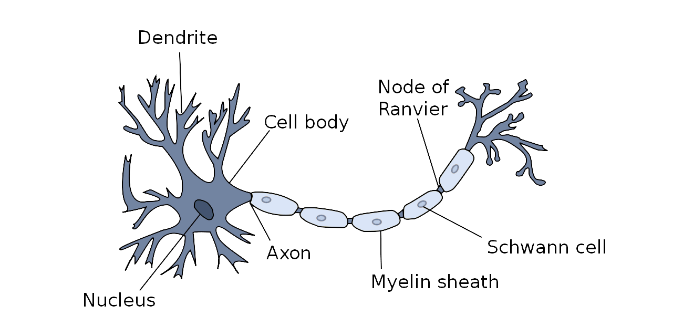
\includegraphics[width=0.6\textwidth]{images_miscelaneus/neuron.png}
\caption{Biological Neural Network. Image obtained from \cite{BINN}} \label{fig:Bio-Neuron}
\end{figure}

The soma is the spherical central part of the nerve cell in whose there is a salt and potassium concentration which is covered by the neuronal membrane. Inside the soma is the neuronal nucleus and from the soma branches are extend (dendrites). Nerve cells are connected among them by dendrites. Neurons are transmitting and receiving nervous signals continuously, communicating among them. The information transference is produced, more specifically, in the synaptic clef (space between two neurons connection). This exchange of information is denominated synapses and it is made though electrochemical activities. The axon is a soma extension whose responsibility is transmitting the information electrochemical out of the neuron, by the nervous system thanks to its terminal branches \cite{BINN, neuroscience}\\

\subsection{Artificial Neural Networks (ANN)}
As the same way as the nervous systems is formed by neurons, artificial neural networks are composed by artificial neurons. Each artificial neuron is a processing unit whose input is processed and shared to another neuron or to the output. Neurons are connected among them \cite{BINN}\\

Basically, there are three types of artificial neurons:
\begin{description}[noitemsep,topsep=8pt,parsep=0pt,partopsep=20pt]
\item \textbf{Input neurons}, if belong to the input layer. This neurons receive the input data of the network.\\
\item \textbf{Hidden Units}, if belong to the processing layers. There are many types of layers: convolutional, pooling, dropout... There could be as many hidden layers and hidden units as user desire. The connectivity and the topology of the layers define the topology of the network. \\
\item \textbf{Output neurons}, if belong to the output layer. This neurons gives the user the processed information.\\
\end{description}

In figure \ref{fig:esquemaneuronal} the schematic of a general neural network it is possible to visualize the schematic of a general neural network with an undefined number of neurons in each layer and an undefined number of hidden layers.\\

\begin{figure}[htb]
\centering
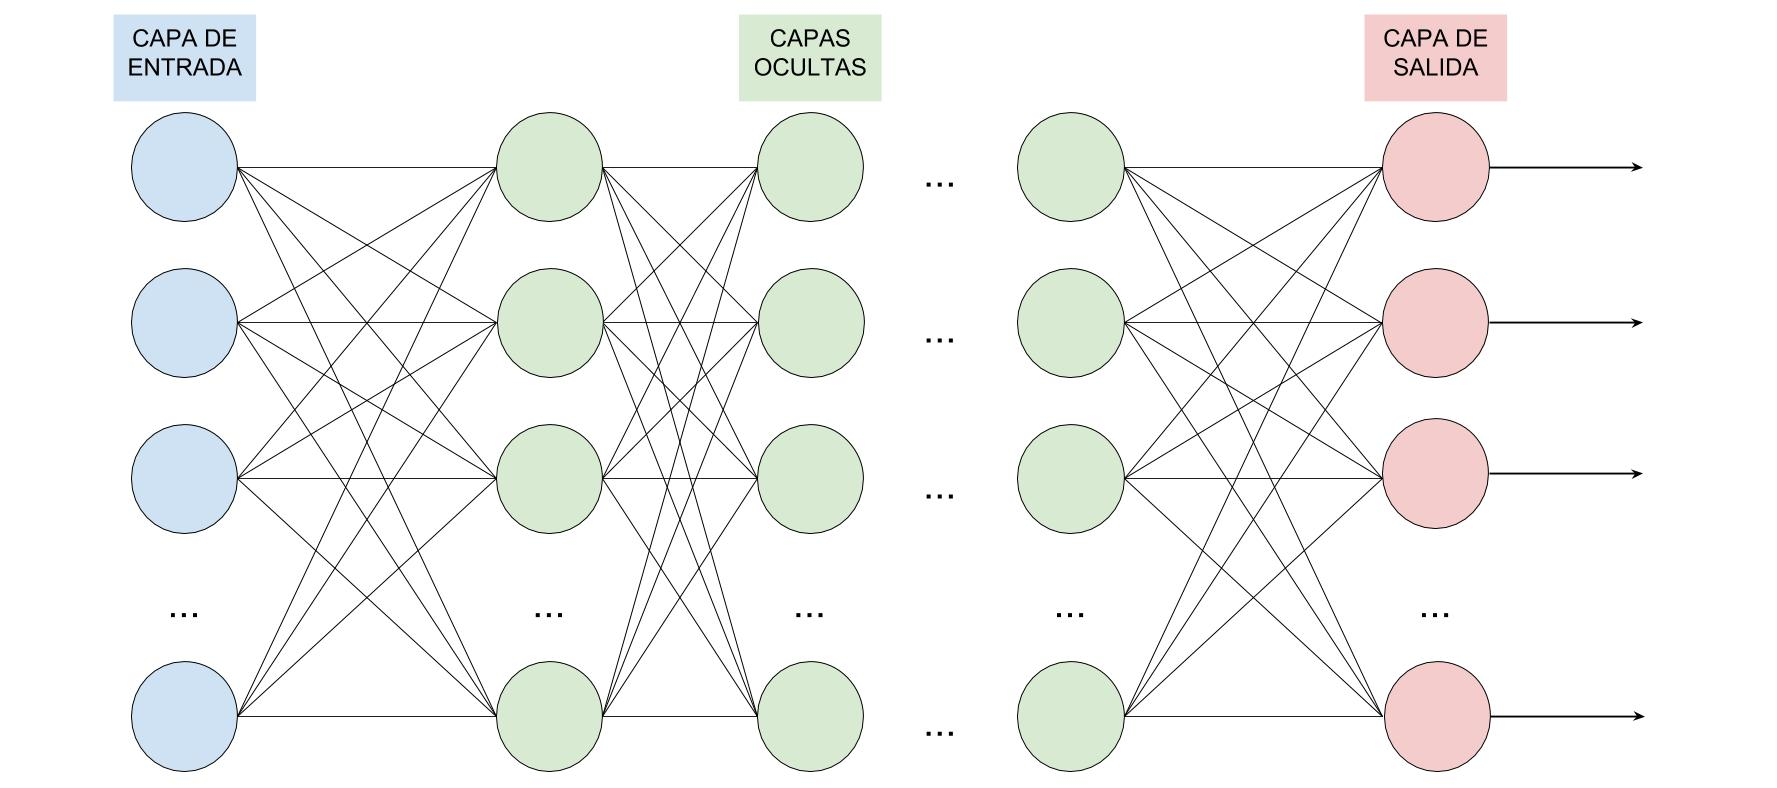
\includegraphics[width=0.55\textwidth]{images_miscelaneus/red_neuronal.jpg}
\caption{Schematic of a general neural network.} \label{fig:esquemaneuronal}
\end{figure}

A single neuron is formed by an input, a weight \textit{W} and a bias \textit{b} associated (Independent term). The value of the bias is always 1, but it has an associated weight that maked that the value of the bias change. Weight and bias values could be modified. The output of the neuron is associated to an activation function. \\

\begin{figure}[htb]
\centering
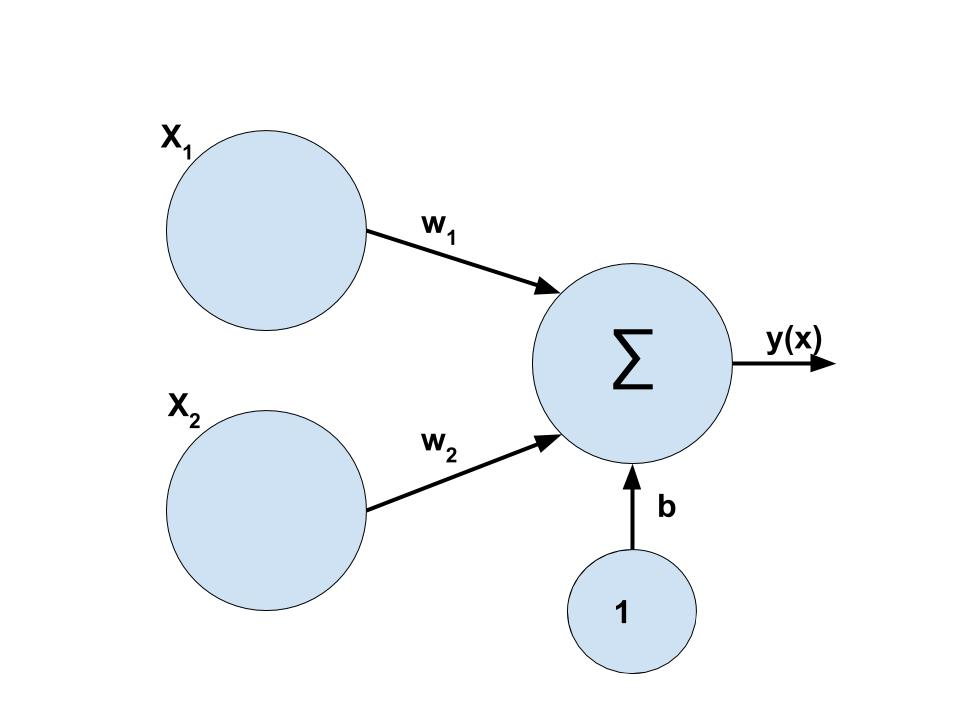
\includegraphics[width=0.55\textwidth]{images_miscelaneus/neurona_sencilla.jpg}
\caption{Simplest neural network architecture.} \label{fig:neuronasencilla}
\end{figure}

The simplest example of a neural network is formed by two inputs neurons and a output neuron as it is shown in figure \ref{fig:neuronasencila} in which \textit{$W=[w_1,w_2]$} are refered to the weights assigned to each neuron. The \textit{b} value is refered to the bias term. \textit{$X=[x_{1},x_{2}]$} are the input of the network architecture and \textit{y(x)} the output. The output is predetermined by the equation \ref{eq:ecuation_neuronasencilla}. So, the output would depend on the input, weights and bias sand the activation function \textit{F} \cite{krose} and it would result as he transfer function.\\

%Ecuacion salida neurona
			\begin{equation}
			y(x)=F(\sum_{i=1}^{2} (w_{i}*x_{i} + b) )
			\label{eq:ecuation_neuronasencilla}
			\end{equation}\\


Due to activation function, the output of the neuron would change if the input is bigger than a some threshold. This threshold is defined by the own activation function. There are various functions that are used: sigmoid function, Heaviside function, Fermi function or hyperbolic tangent among others. In figure \ref{fig:activation_function} (which has been obtained from \cite{BINN}) the mentioned function are shown and the output would be 0 or 1 values if the function is sigmoid or Fermi and the output would be -1 or 1 if the function is an hyperbolic tangent. \\

\begin{figure}[htb]
\centering
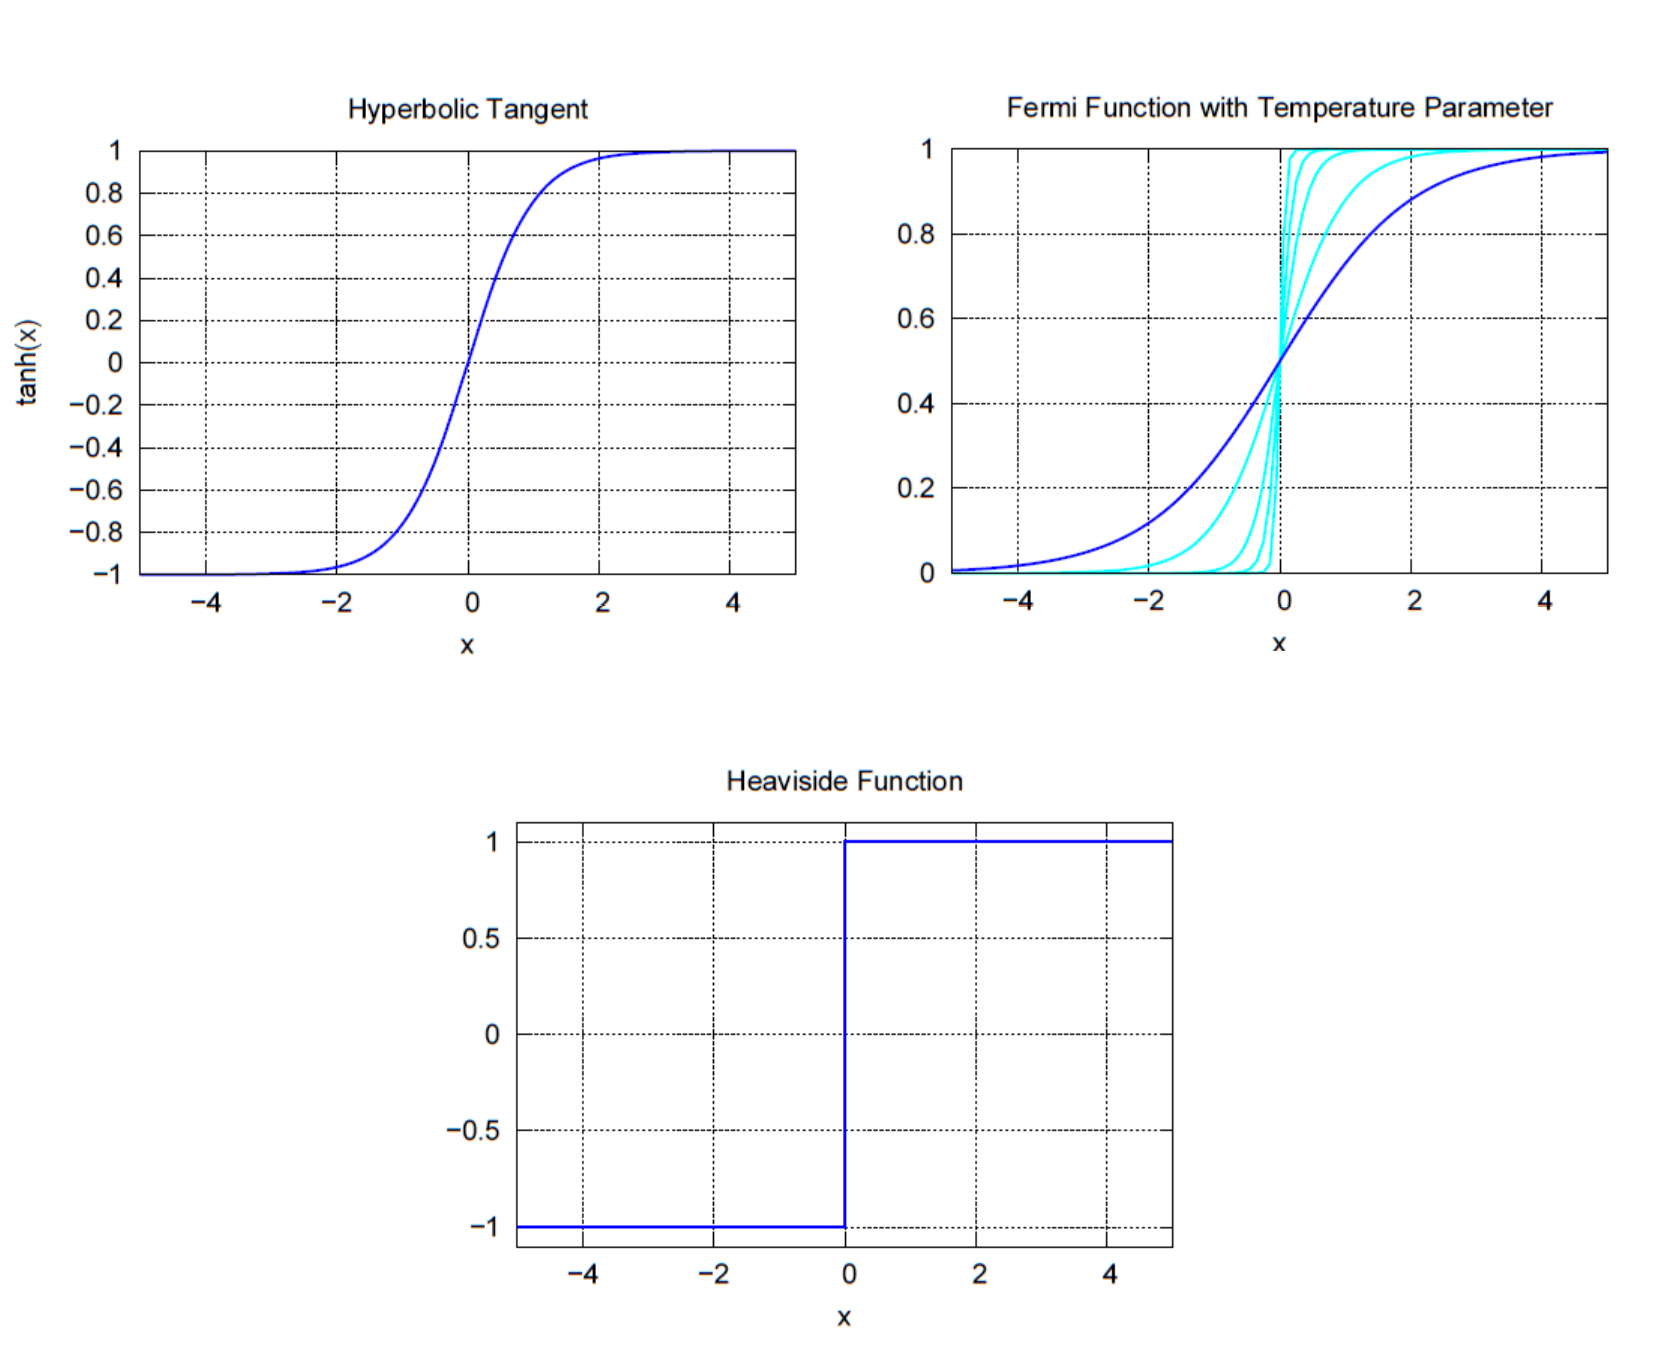
\includegraphics[width=0.55\textwidth]{images_miscelaneus/activation_function.PNG}
\caption{Different activation functions. Image obtained from \cite{BINN}} \label{fig:activation_function}
\end{figure}

\subsubsection{Analogies between ANN and Biological Neural Networks}
Analogies between Artificial and Biological Neural networks could be found (if both basic theory is known) because the first one (artificial NN) are based in the second one. It is easy to see that biological neurons correspond to artificial neurons. But the cell body correspond with transference function. The output to others neurons would correspond to the axon and synapses with weights and bias. The soma would correspond with the transfer function. Those analogies are summarized in table \ref{Analogias}. Artificial neural networks are just inspired in Biological neural networks, that both work in a different (although inspired) way must be made clear.\\

\begin{table}[h]
\centering
\begin{tabular}{|c|c|}
\hline
\rowcolor[HTML]{ECF4FF} \textbf{Artificial Neural Component} & \textbf{Analogy}        \\ \hline
Neuron Artificial Neuron                        & Biological Neuron       \\
Transfer function                & Soma \\
Connexion between Artificial neurons               & Axón                     \\
Weight                                     & Synapses                 \\ \hline
\end{tabular}
\caption[Analogies between artificial neural networks and biological neural networks]\label{Analogias}
\end{table}
